\chapter{Wykład 4. Zarządzanie wiedzą w przedsiębiorstwach}

\section{Procesy wykorzystania produktu projektu}
% strona 34

Zobacz Rys.~\ref{fig:opracowanieWBS}~i~\ref{fig:zarzadzanieRyzykiem}.

\begin{figure}[hbt]
\centering
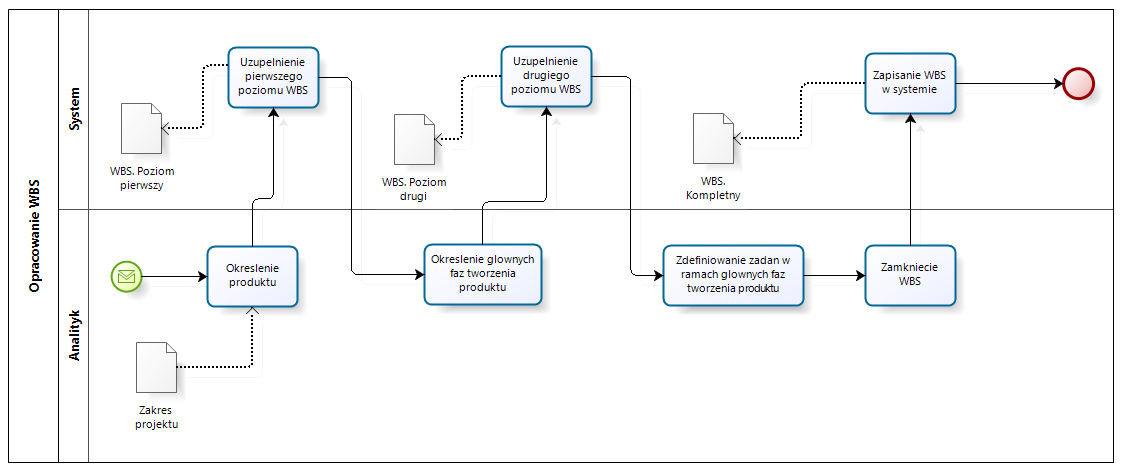
\includegraphics[width=1.1\textwidth]{opracowywanieWBS.png}
\caption{Tworzenie WBS}
\label{fig:opracowanieWBS}
\end{figure}

\begin{figure}[hbt]
\centering
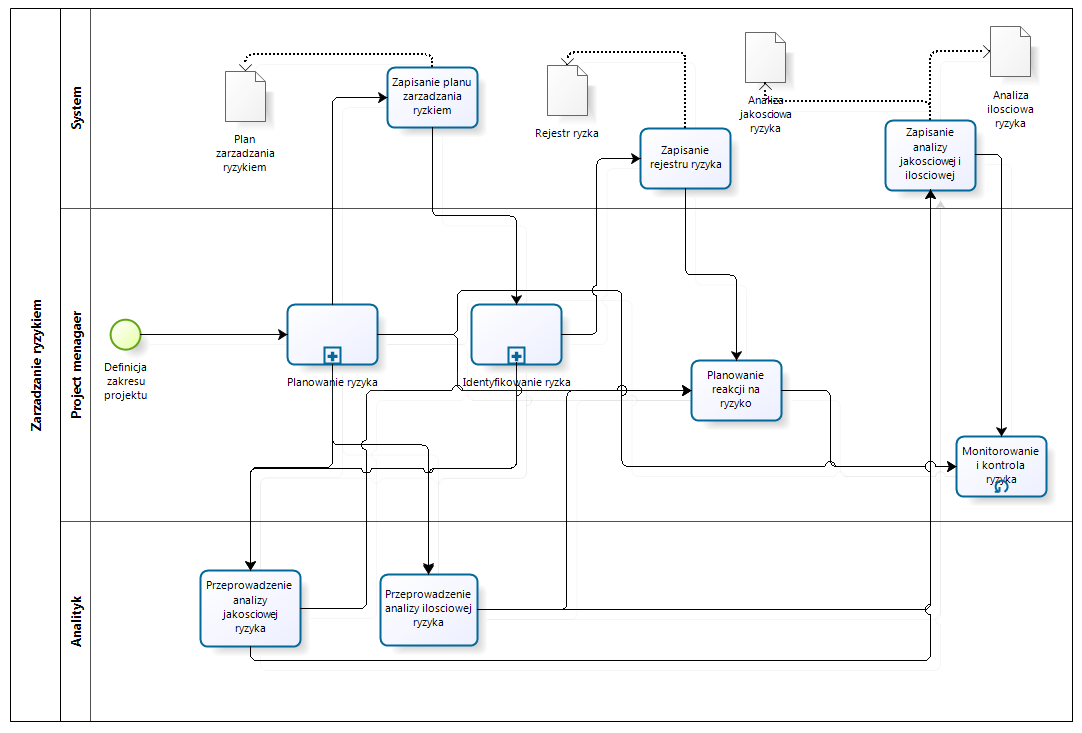
\includegraphics[width=1.1\textwidth]{zarzadzanieRyzykiem.png}
\caption{Zarządzanie ryzykiem}
\label{fig:zarzadzanieRyzykiem}
\end{figure}

% ===========================================================================

\section{Model przepływu danych}
% strona 40

Ten wirtualny warsztat jest beznadziejny.

% ===========================================================================

\section{Mapa umysłu dla systemu zarządzania wiedzą}
% strona 70

Zobacz Rys.~\ref{fig:mapaMysli}

\begin{figure}[hbt]
\centering
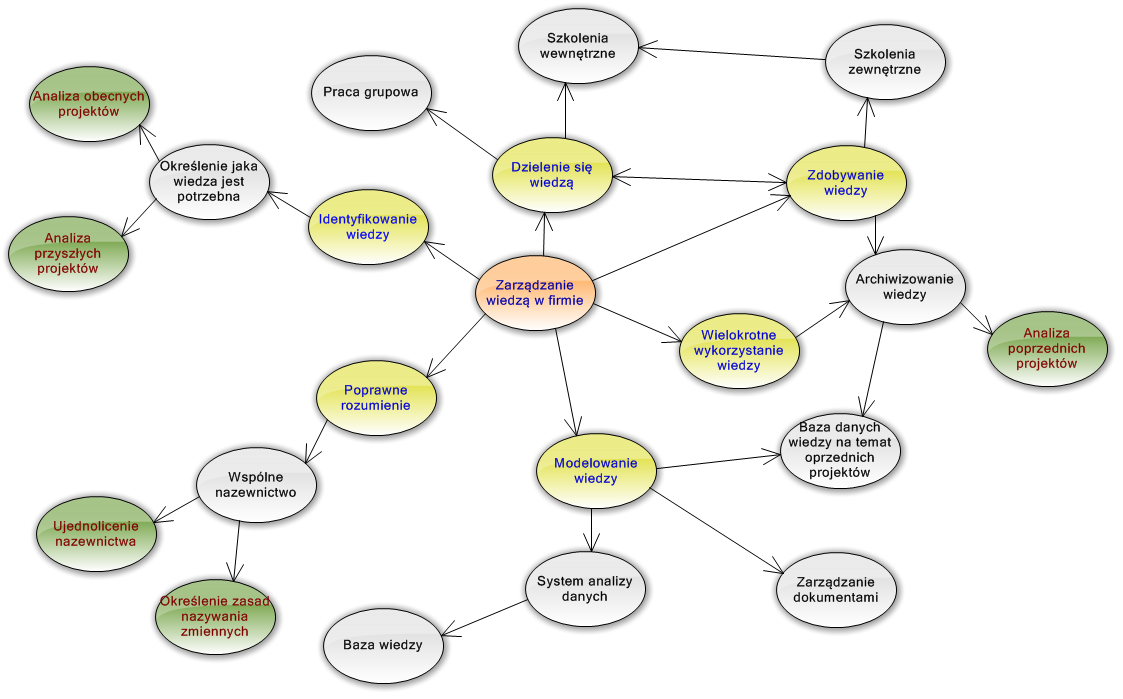
\includegraphics[width=\textwidth]{mapaMysli.png}
\caption{Mapa myśli}
\label{fig:mapaMysli}
\end{figure}

% ===========================================================================

\section{Przegląd praktyk OPM3}
% strona 89

Praktyki OPM3, które powinny być w firmie:

\begin{enumerate}
\item Integrate PMBOK Guide Knowledge Areas; z racji związania projektu z metodyką PMBOK
\item Project Team Development Process Measurement; w związku z pracą zespołową nad projektem
\item Project Risk Response Planning Process Control; związane z występowaniem ryzyka
\end{enumerate}

Praktyki OPM3 zbędne w firmie:

\begin{enumerate}
\item Know Inter-Project Plan; w trakcie trwania projektu nie będą prowadzone równolegle inne projekty
\item Optimize Portfolio Management; brak portfolio
\item Track the Return of Investment; projekt nie jest inwestycją firmy
\end{enumerate}

